\documentclass{article}
\usepackage[utf8]{inputenc}
\usepackage{graphicx}
\usepackage{hyperref}
\usepackage{minted}


\begin{document}

\title{How To Sigi}
\author{Ekter}
\date{August 2024}
\maketitle


\section{Introduction}

The Sigi is a robot from Pololu(the Balboa 32U4 board) combined with a Raspberry Pi.
It is a segway-based robot(inverted pendulum on wheels), so it has two parallel wheels.
It is an unstable system, so it is interesting to try the stability of different controllers.

This document is a guide to how to use the Sigi robot.
It attempts to be a comprehensive guide to the robot, from the hardware to the software,
including various useful resources for understanding the operation of all different parts of the system.
It will also include some info on problems caused by the current design of the system and,
when possible, details on how to fix them.

If detailed documentation is needed, the \href{file://other_doc/Sigi_documentation_part1.pdf}{Sigi2.0: Documentation}
is quite complete on anything related to hardware.


\section{Hardware}

\subsection{Different parts overview}
\subsubsection{Balboa 32U4}
The Balboa 32U4 is the main board of the robot.
It can be programmed like an Arduino board using the Arduino IDE for example, by plugging the board to a
computer using its micro-USB interface.
It has a lot of components, but the most important are:
\begin{itemize}
    \item The two motor drivers, which are used to control the two motors of the robot.

    \item The IMU, which is used to measure the angle of the robot.

    \item The encoders, which are used to measure the speed of the motors.
\end{itemize}

Other notable components are:

\begin{itemize}
    \item The buzzer, which can be used to make sounds.

    \item The buttons, which can be used to interact with the robot.

    \item The LEDs, which can be used to show information to the user.

    \item The battery monitor, which can be used to measure the battery level.

    \item The communication interfaces and GPIOs, which can be used to connect the board to
        other devices.

    \item A reset button on the side of the board.
\end{itemize}

\subsubsection{Raspberry Pi3B+}
The Raspberry Pi are a series of small single-board computers.
The Raspberry Pi 3B+ is the one used in the Sigi robot.
It is used to run the high-level software of the robot.

The Pi 3B+ in particular features a wi-fi interface which can be used to connect to the robot
remotely.

\subsection{Sigi power management}
The Sigi is intended to be used with cells, but can also be powered by its micro-USB interface,
with an USB power bank for example.
But the micro-USB interface is not fed into the motors, so a jumper wire has been installed on the
Sigi bypass the battery regulator and feed the motors with the micro-USB power when connected.
This jumper is located between the VSW and the 5V pins near the micro USB port of the Balboa board.

\begin{center}
    % \begin{figure}                % I don't know how to use this
        
        
        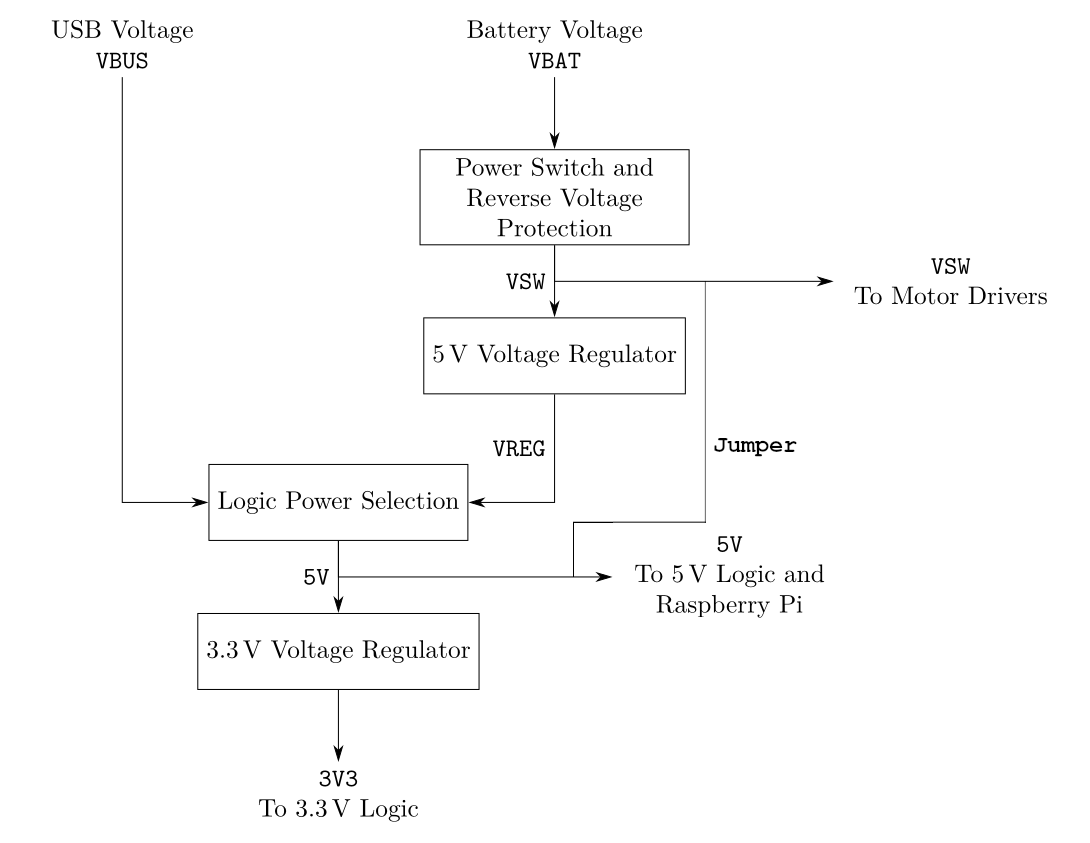
\includegraphics{img/power.png}

        Figure 1: The jumper wire on the Sigi robot voltage lines.
    % \end{figure}

\end{center}

This is fine most of the time, but it can occasionally cause problems.
If the current drawn by the system is too high(high speed change in the motors+heavy 
computations on the Raspberry Pi), the voltage of the 5V logic will drop, causing
resets of the Balboa board. Fortunately this reset stops the motors, so the voltage will rise
again, so the Raspberry Pi, requiring less voltage, won't reboot. But since the Balboa board
resets, the encoders will reset, which may cause the robot to lose its position if it was not
saved by the Raspberry Pi.

One solution could be using a battery, but the jumper prevents the battery's voltage from being
too high, since it is connected to the 5V logic and the Raspberry Pi. Experimentally, the max
voltage was measured around 7.5V, but it was already causing consumption and heating problems on
the regulator. In normal conditions, the voltage should be capped at 7V for safer operation.
This also implies a minimal voltage. In fact, the voltage protection removes approximately 10\%
of the voltage, so in order to achieve the 5V logic, the voltage should be at least 5.5V.
Some problems have been observed at 5.5V, but their exact cause is unknown. It could be the
voltage regulator not having enough power when the motors are running for example.
So the optimal voltage of a battery should be between 6 and 7V. A higher voltage battery
with a voltage regulator would also be ok.

*note: insert power diagram

Removing the jumper would help if using a battery, but of course it would prevent to go back to
using an USB power bank without soldering the jumper back.

Side note:
It is what I have done with my Sigi(14), and I alternate between the battery and the USB power
for tests and operation.

Another solution could be to use another Raspberry Pi with less current consumption. For example,
a Pi Zero W has almost the same wireless capabilities, but consumes less power. However,
the computational power is also reduced, so it may not be enough for some applications.

\section{Software}
The current design of the Sigi is like this:

\begin{center}

    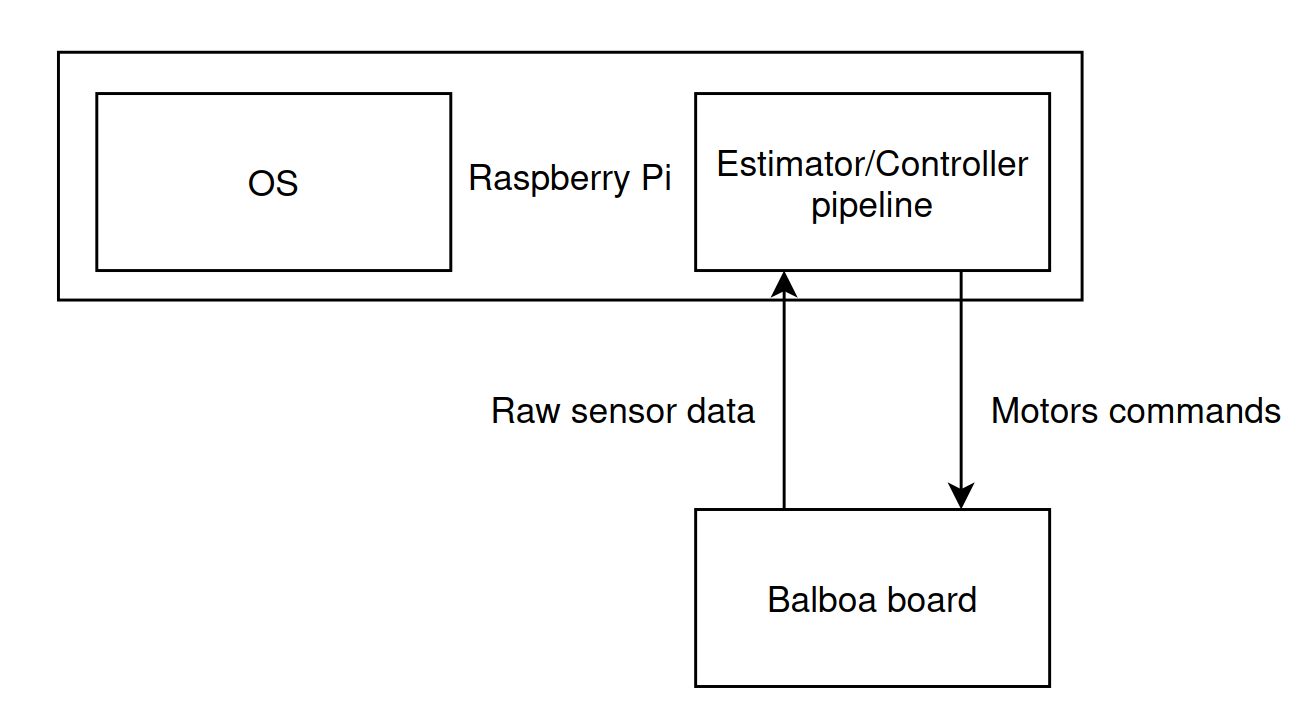
\includegraphics[scale=0.2]{img/software.png}

    Figure 2: Software overview

\end{center}

The Balboa 32U4 is only used to get the raw sensor data, and the controller is running on the
Raspberry Pi. The Balboa board could also be used to run the controller, but using the Raspberry
Pi allows for more complex computations and easier debugging. The possibility of using the Python
language is also a plus, see 3.3 for more details.

\subsection{Interface between the Raspberry Pi and the Balboa board}

Communication between the Raspberry Pi and the Balboa board is needed for multiple purposes
that cannot be done directly with the Raspberry Pi :

\begin{list}{-}{}
    \item Reading the state of the robot from the sensors
    \item Sending commands to the motors, LEDs or other actuators
\end{list}

The communication is done via the I2C interface.
Other communication media could possibly be used, but have not been documented by Pololu,
using an USB or UART interface for example.
The current protocol used is actually a variant of the I2C protocol, the
\href{https://en.wikipedia.org/wiki/System_Management_Bus}{SMBUS} protocol.
The Raspberry Pi is the master and the Balboa board is a slave.
The IMU is also a slave, since it is accessed directly by the Raspberry Pi without
going through the Balboa board's micro controller.

\begin{center}

    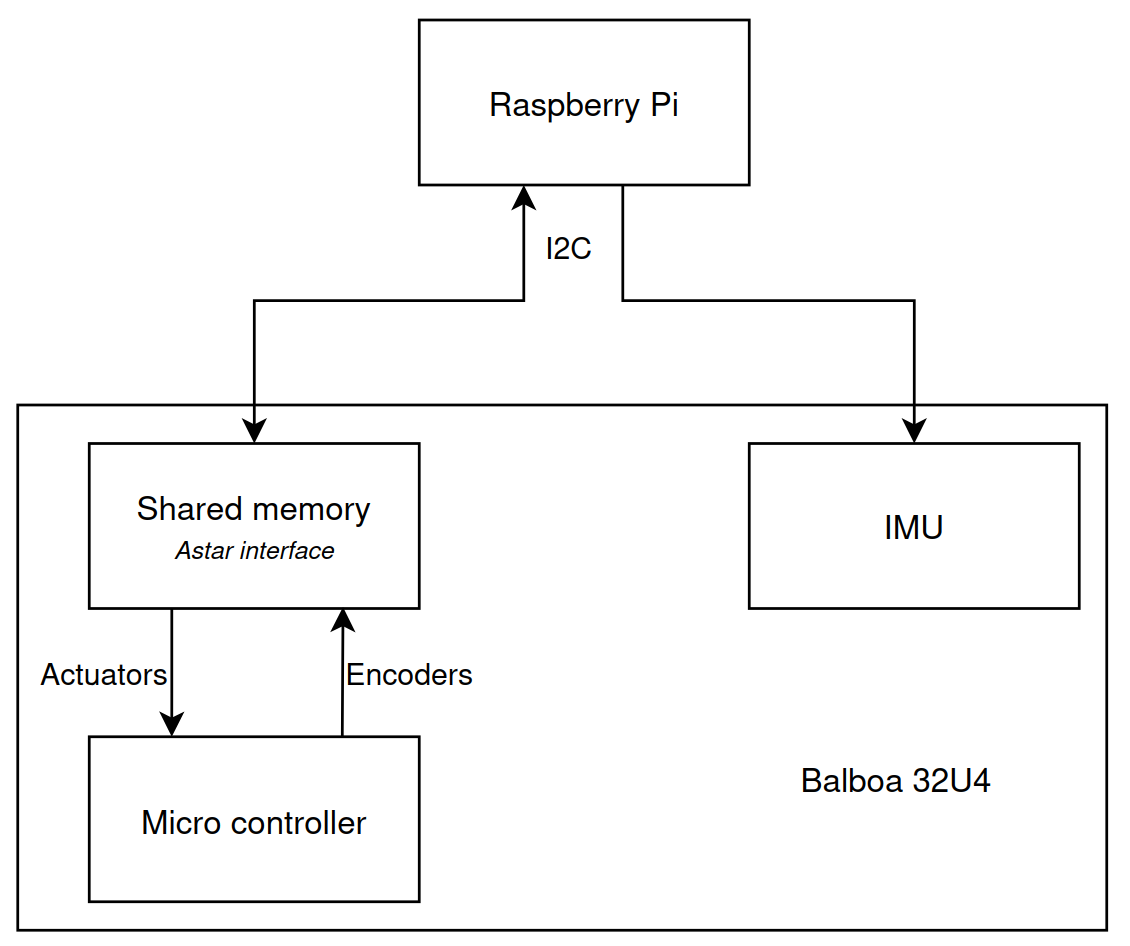
\includegraphics[scale=0.25]{img/i2c-interface-diagram.png}

    Figure 2: I2C diagram of the Balboa/Pi interface
    % TODO make this correctly(shared memory etc)

\end{center}

\subsubsection{Balboa board}

The Balboa board's micro-controller has to read the shared memory(note: it is called a buffer in
the code but it is technically not one) to know the orders from the Raspberry Pi, and update its
right fields so that the encoders ticks can be read from the Raspberry Pi.
The default example code from Pololu handles these tasks quite well. A notable possible
improvement could be improving it to read the last saved value on the buffer after resets to
recover more efficiently. It could also be possible to write more information in the buffer, like
debugging information.

The default example code can be found in the
\href{https://github.com/pololu/pololu-rpi-slave-arduino-library/blob/master/examples/AStarRPiSlaveDemo/AStarRPiSlaveDemo.ino}
{Pololu's GitHub repository}.
It can easily be flashed on the Balboa board using the Arduino IDE.

\subsubsection{Raspberry Pi}

The Raspberry Pi has to access the shared memory to read the encoders ticks and write the orders.
The best way to do it is simply using the Raspberry Pi's I2C interface.

Pololu recommends using their Python library to communicate with the Balboa board. It can be found in
\href{https://github.com/pololu/pololu-rpi-slave-arduino-library/blob/master/pi/a_star.py}{their Github}
as well as the example code.

It is possible to use the I2C interface directly, but it is more complicated and error-prone.
The exact addresses to read and write are documented here: \href{file://other_doc/Sigi_documentation_part1.pdf}
{Sigi2.0: Documentation}.


\subsection{Operating System of the Raspberry Pi}

Since the Raspberry Pi only has to use its I2C interface to communicate with the Balboa board,
any OS that supports I2C can be used.

The two main possibilities are the Raspberry Pi OS, a Linux-based OS very similar to Ubuntu
(it is derived from Debian), and the Matlab OS form Mathworks.

The Matlab OS would have been very interesting since it allows to run Matlab/Simulink models
in real time, but its I2C interface seems to be broken. The previous students have demonstrated
that every time the Matlab OS tried to read a value from the shared memory, using the I2C
functions of the matlab OS, it started by setting the values of the whole memory array(next 8
addresses) to full 1. This typically caused the robot to start playing the Fugue every time an
attempt to read the encoders was made, and would read false values (full 1).
This bug could maybe be fixed, but since the matlab OS doesn't let full control over the system,
it could be hard and would certainly require a lot of time.

So for now, the Raspberry Pi OS is the best choice.
See the section 4 for details on how to install it.

\subsection{Programming language}

It is possible to use almost any language on the Raspberry Pi, but Matlab would be really hard
to install because they do not support ARM processors, and the RAM of the Pi is way too low (see
\href{https://fr.mathworks.com/support/requirements/matlab-linux.html}{Matlab on Linux requirements}).

Python seems to be the optimal choice, because it has a great support for Raspberry Pi.
It is also a great language for prototyping, and it is easy to use.
However, it is not the fastest language, it is interpreted, and has an irregular garbage
collection system, so it is not precise in terms of time.

It could be possible to use C or C++, but it would be harder to use.

\subsection{Software architecture}

Now that we know the OS and the programming language, we can focus on the software architecture.
The python code is based on ftprci, a Python library developed for this occasion, that can also
be used for other projects.

\subsubsection{ftprci presentation}
\href{https://github.com/Ekter/ftprci}{ftprci} mean "Fast Time Robot Controller Interface". It is designed to be a fast and easy to use
interface to control robots. The goal is to regroup different pieces of code that are often used
in robot controllers, like the PID controller, the Kalman filter, the LQR controller, etc. in a
single library. It is also designed to be easy to use, with a simple API.

The library is still in development, but it is already usable.

To use the library, the principle is to implement diverse classes needed for the robot, like an
estimator, a sensor interface\dots
Some classes are already implemented, like the PID controller, some sensors\dots

The library also has a low level part to control timings precisely to ensure that the loop runs at
the right frequency with as little jitter as possible.

But if you have to implement a new class, you should follow the ftprci interface.
Here is the UML diagram of the library:

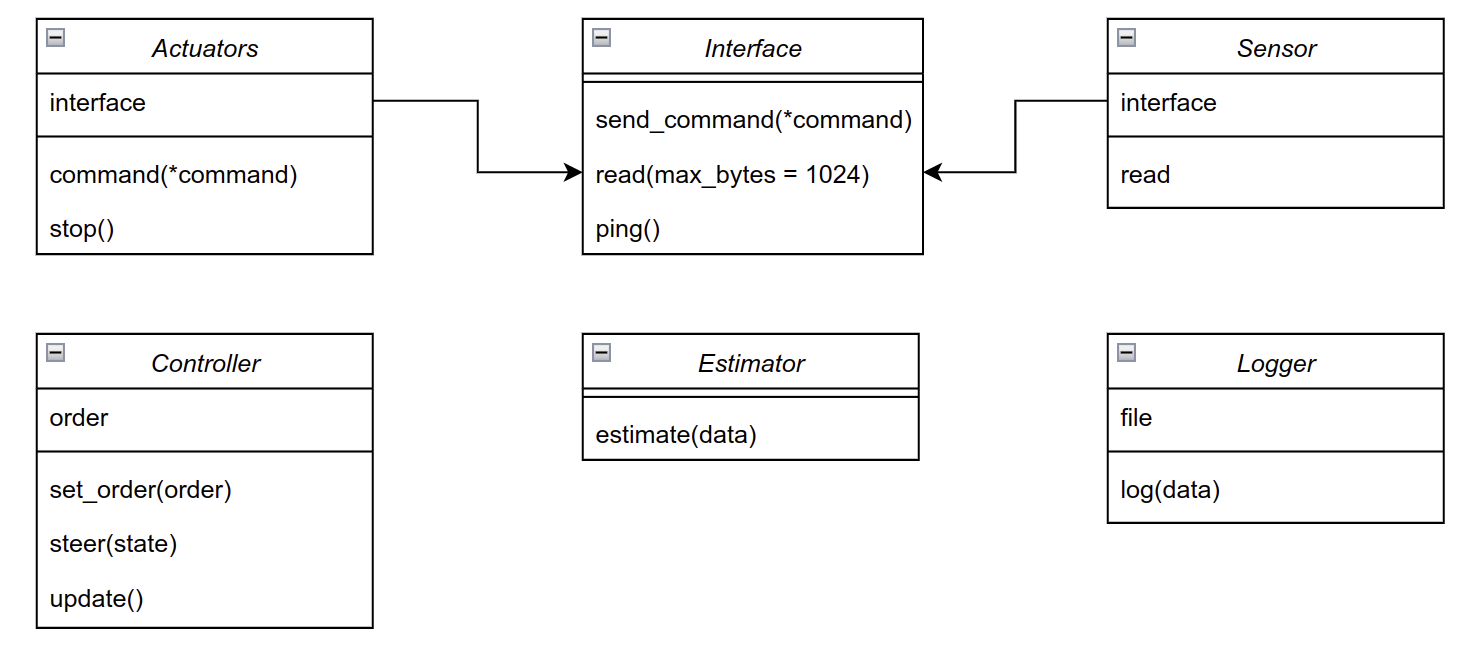
\includegraphics[scale=0.2]{img/uml_ftprci.png}

Controlling the Sigi using ftprci is trivial, because all necessary classes are already
implemented. This really simplifies the code, and makes it easier to understand.

When you have your classes ready, you can start to link them. Basically, the normal architecture
should be :

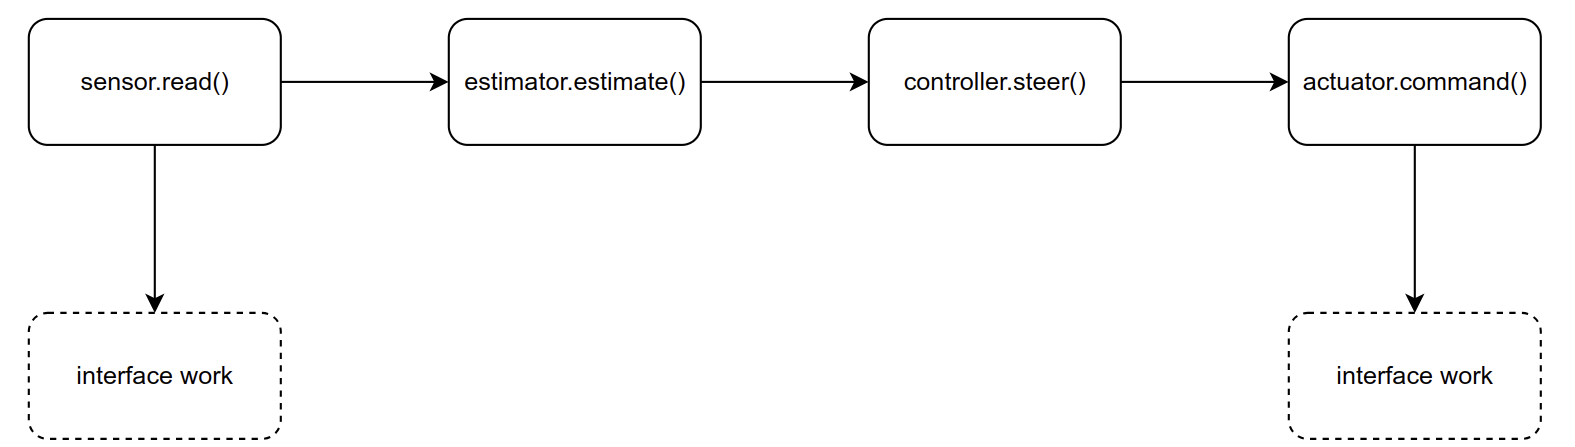
\includegraphics[scale=0.2]{img/gen_flowchart_ftprci.png}

This is what the code should look like. Everything else is handled by the library, including
the management of the loop, the threading part, and so on.
Basically, the library creates a thread for running the loop, and the above diagram is run as
the callback in the loop.
This means that the code can be controlled from the main thread, while
the loop is running in another thread.
Any function can be used as a callback, which makes it easy to add new functions. For example, if
logging the output of the estimator is needed, it can be added in the middle callback.

Every function added to the callback will be executed, and their output will be sent to the next
function. This is a simple way to chain functions.

For the Sigi, the code looks like this:

\inputminted[linenos]{python3}{../main.py}

The first line imports the library.

The next 4 lines instantiate the classes needed: the LSM6 (with an address of 0x6B), the
complementary filter, the PID controller, and the Pololu Astar actuator controller.

The 12th line instantiates the runner thread and starts it, with an empty callback.

Then the next line defines the callback of the loop. You can notice it is exactly the same as the
flowchart above.
So the functions of the callback will start to get executed.

The while loop only gives orders to the controller to make the Sigi move around.

This simplicity is the advantage of this library: you only have to implement the classes you need,
and the library does the rest.

\subsubsection{Implementing a custom class in ftprci}

To implement a custom class in ftprci, you have to follow the interface of the library.
The simplest way to do it is to inherit from the class you want to and re-implement the necessary
methods from the UML diagram.

For example, we will implement a simple updating PID controller. We will inherit from the PID
controller, and overload the update method.

\begin{minted}[linenos]{python3}
class PIDController(Controller):
    def __init__(self, p, i, d, integrator: DiscreteIntegral = None, update_rate=0.01):
        super().__init__(p, i, d, integrator)
        self.update_rate = update_rate

    def steer(self, state):
        self.last_state = state
        self.update()
        return super().steer(state)

    def update(self):
        self.p -= (self.last_state-self.order)*self.update_rate
\end{minted}

This is a simple example, but it shows how easy it is to implement a new class in ftprci.

I will write a proper documentation for the library soon, but for now if you have any question,
do not hesitate to ask me on the ftprci Github via issues for example.

\subsection{Software problems}
% TODO

i2c is slow


\section{Starting with the Sigi}

Starting to work with the Sigi can be quite hard, primarily because of its age.
If the Sigi you have has already been used, you will probably not have to follow this whole
section entirely, so I advise you to just do the checks for every subsection.

However, your Sigi may have been flashed with a very old version of the Raspberry Pi OS, as it was
the case for me. In this case, you may have trouble installing various software, like the vs code
server, or some python libraries for mathematical computations like Clarabel.

\subsection{Hardware}

Let's start by checking the hardware of the Sigi.
The first important thing to check is the power source of the Sigi.
If you use an USB power bank, is it charged?

If you chose to use an other battery to power the Sigi as I've advised in the power management
section, is it correctly connected to the battery input pins of the Balboa board?

It can also be interesting to check if you have the jumper wire on the Sigi, and if it is soldered.
It should be on the upper part of the board, between the VSW and the 5V pins, on the side near the
Raspberry Pi. If you do not have it, you won't be able to use the power bank to power the motors,
but you can continue for now.

\subsection{Balboa board's firmware}

You can flash the firmware using the Arduino IDE, and the code can be found in the
\href{https://github.com/pololu/pololu-rpi-slave-arduino-library/blob/master/examples/
AStarRPiSlaveDemo/AStarRPiSlaveDemo.ino}{Github of Pololu}.
The insctructions to flash the firmware are here : \href{https://www.pololu.com/
docs/pdf/0J70/balboa_32u4_robot.pdf}{Pololu Balboa 32U4 Balancing Robot User's Guide}

\subsubsection{Check}
If you have flashed the firmware, you can check if it is working by turning the Sigi on
(connecting the micro USB to the power bank or the battery). If the code is flashed correctly, then
a sound will be played.

This sound is played at every reset of the Balboa board.
You can disable it if you find it annoying by commenting the line 56 of the example code, but I
advise you to keep it for now because it is a good troubleshoot tool. In fact, resetting the Balboa
board will reset the encoders, so if you hear the sound, you know that the encoders have been
reset.

\subsection{Raspberry Pi SD card flashing}

We will remove the Raspberry Pi from the Sigi for the next part.

We need to connect the SD card of the Raspberry Pi to a computer to flash the OS.

There are two main possibilities to flash the Raspberry Pi OS: using the Raspberry Pi Imager, or
manually with an other software like Etcher.

\subsubsection{Using the Raspberry Pi Imager}

\href{https://www.raspberrypi.com/software/}{Raspberry Pi Imager} is a software that allows you to
flash the Raspberry Pi OS on an SD card easily.
It automatically downloads the OS, flashes it on the SD card, and verifies the flashing.
It also allows you to setup some settings like the wifi connection, etc.

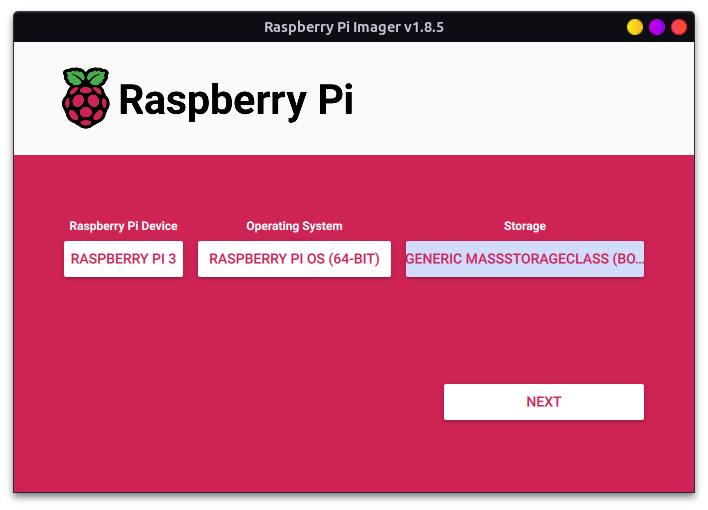
\includegraphics[scale=0.4]{img/imager_next.png}

After downloading the imager, the process is quite simple:

\begin{itemize}
    \item Select Raspberry Pi 3 for the device.
    \item For the operating system, choose Raspberry Pi OS Lite, 64bits if possible. It may be in
        the category "Raspberry Pi OS (other)".
    \item Select your SD card on the list of storages. Warning: it will be formatted, so make sure
        you have selected the right one. Unplugging it from the computer will remove it from the list,
        so you can check like this.
    \item Edit settings : you can set the wifi connection here, it should help later. I also advise
        you to enable SSH, so you can connect to the Raspberry Pi remotely, and to create a ssh key to
        login without password. Github has a good \href{https://docs.github.com/en/authentication/
        connecting-to-github-with-ssh/generating-a-new-ssh-key-and-adding-it-to-the-ssh-agent#
        generating-a-new-ssh-key}{tutorial} on how to do it.
        I recommend you to set the username to sigi<number of your sigi> to be able to connect easily.
    \item Click yes to apply the settings.
    \item Wait for the flash to finish, it should take a few minutes depending on the size of the
        SD card and your internet connection if you do it for the first time.
\end{itemize}

\subsubsection{Using BalenaEtcher}

It is also possible to flash the Raspberry Pi OS using \href{https://etcher.balena.io/
}{BalenaEtcher}, or any other software that can flash an image on an SD card, like Rufus.

BalenaEtcher is used here as an example, but the process is quite similar with other software.

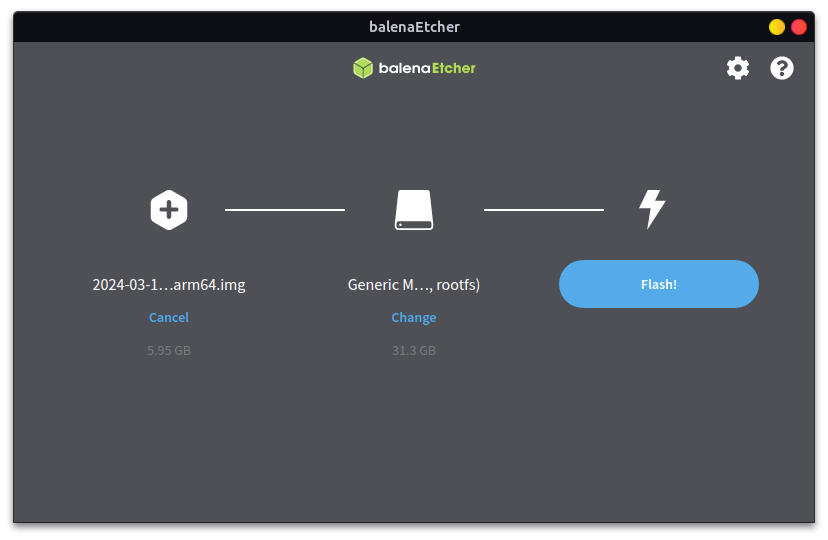
\includegraphics[scale=0.3]{img/etcher_next.png}

To flash the OS with Etcher:
\begin{itemize}
    \item Download the right image of the Raspberry Pi OS from the
        \href{https://www.raspberrypi.com/software/operating-systems/}{Raspberry Pi website}.
        It should be the Raspberry Pi OS Lite, since we will not use the desktop environment.
        The 64bits version is recommended.
        The download is quite big, so it may take some time.
    \item Choose the image you have just downloaded.
    \item Choose the SD card you want to flash. Warning: it will be formatted, so make sure you
        have selected the right one. Unplugging it from the computer will remove it from the list,
        so you can check like this.
    \item Click on flash.
    \item Wait for the flash to finish, it should take a few minutes depending on the size of the
        SD card.
\end{itemize}

\subsubsection{Check}

To check if the flashing is correct, the easiest way is to read it using a computer.
Opening the Disk Management on Windows, GParted on Linux, or Disk Utility on MacOS should show you
the different partitions of the SD card.
There should be at least two partitions: one boot partition, and one root partition, followed by
free space. If not, the Raspberry Pi will not be able to boot.
Here is an example of what it should look like on GParted:

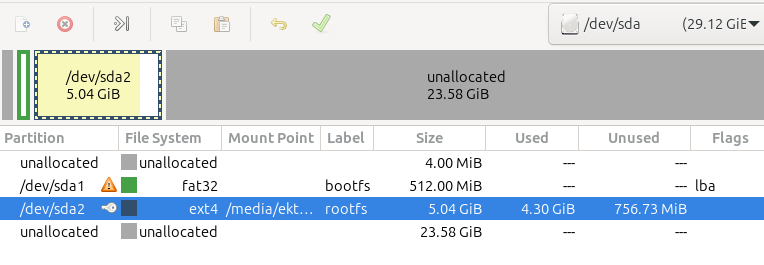
\includegraphics[scale=0.4]{img/partitions_gparted.png}

We can open the root partition on the file browser. The folders should be the typical folders of a
Linux system, like \texttt{bin}, \texttt{boot}, \texttt{dev}, \texttt{etc}, \texttt{home},
\texttt{lib} \dots

Note: it is better to leave the empty space for now, we will change this later. But if it doesn't
work then, you can to expand the root partition using your disk manager.

\subsection{Raspberry Pi setup}

Now that the Raspberry Pi OS is flashed, we can setup the Raspberry Pi.

We need to insert the SD card in the Raspberry Pi, and power on the Raspberry Pi.
The Raspberry Pi should boot, and you should see the leds blinking.

If you have a screen and a keyboard, plug them to the Raspberry Pi, it will be easier to setup the
Raspberry Pi. In this case, you can ignore the next section.

It takes some time for the Raspberry Pi to boot for the first time, so be patient.

For the next steps, you will need to connect to the Raspberry Pi using SSH. Depending on your OS,
you may need to install an SSH client.

\subsubsection{Setting up SSH connection without a screen(more complex)}

If you have enabled the SSH connection in the Imager, you can connect to the Raspberry Pi using
SSH, provided that the Raspberry Pi is connected to the Internet, that you know the IP address of
the Raspberry Pi, and that there is no firewall blocking the connection.

If you can connect both the Raspberry Pi and your computer to the same network, you can use a
command like nmap to find the IP address of the Raspberry Pi.
For example, plugging them both on a switch via Ethernet, or setting the wifi connection on a
mobile phone to share the connection with the Raspberry Pi.

The IP address of the Raspberry Pi is written on the screen during boot, but if you don't have one,
you will have to find it the hard way.

Then, after getting \href{https://www.whatismyip.com/}{your IP address}, you can find the address
of the Raspberry Pi by installing nmap and running the command
\texttt{nmap -sn <your IP address>/24} on your computer.

This will show you the devices connected to the network, and you should be able to find the
Raspberry Pi.
If you see too many devices and can't identify the Raspberry Pi, it may be interesting to use the
OS detection tool of nmap, using the command \texttt{nmap -O <your IP address>/24}, but it is
longer. You may also need elevation rights to use it.

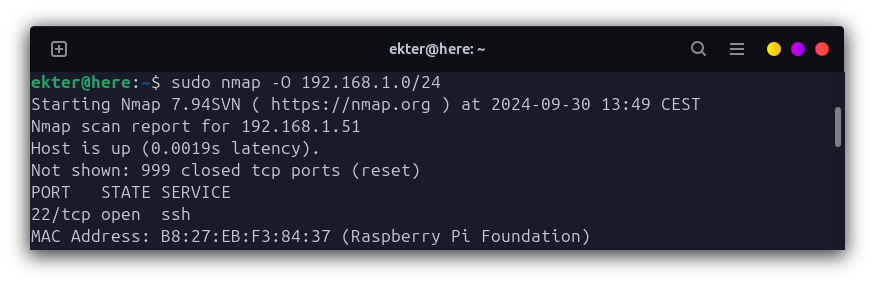
\includegraphics[scale=0.37]{img/nmap_O.png}

To use the ssh command to connect, you also need the username. If you have changed the username in
the Imager, you should use it here. Otherwise, the default username is \texttt{pi}, and the default
password is \texttt{raspberry}. The command to connect is \texttt{ssh <username>@<IP address>}, and
you will be asked for the password if you haven't generated an ssh key.

If the command works, you should be connected to the Raspberry Pi. You have access to the terminal
so you can run commands.
You can skip the next section, and go directly to the next part.

\subsubsection{Setting up SSH with a screen}

If you have a screen and a keyboard, you can setup the Raspberry Pi easily.

After the Pi has finished booting, you should see a login prompt. The default username is
\texttt{pi}, and the default password is \texttt{raspberry}. If you have changed it using the
Imager, use the new username and password.

The first thing to do is to connect the Pi to the internet, or at least, to the same network as
your computer. You can use the command \texttt{sudo raspi-config} to do this if you haven't done
it in the Imager.

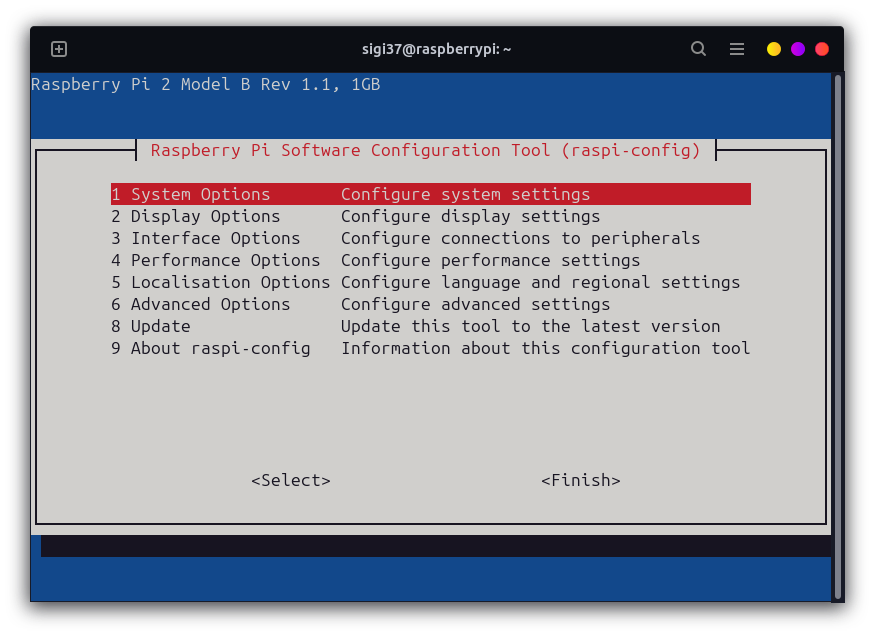
\includegraphics[scale=0.37]{img/raspi_config_home.png}

note: this is not the correct Pi model, I don't have the correct one for now.

It is the first option in the system panel, and you can follow the instructions to connect to the
wifi.

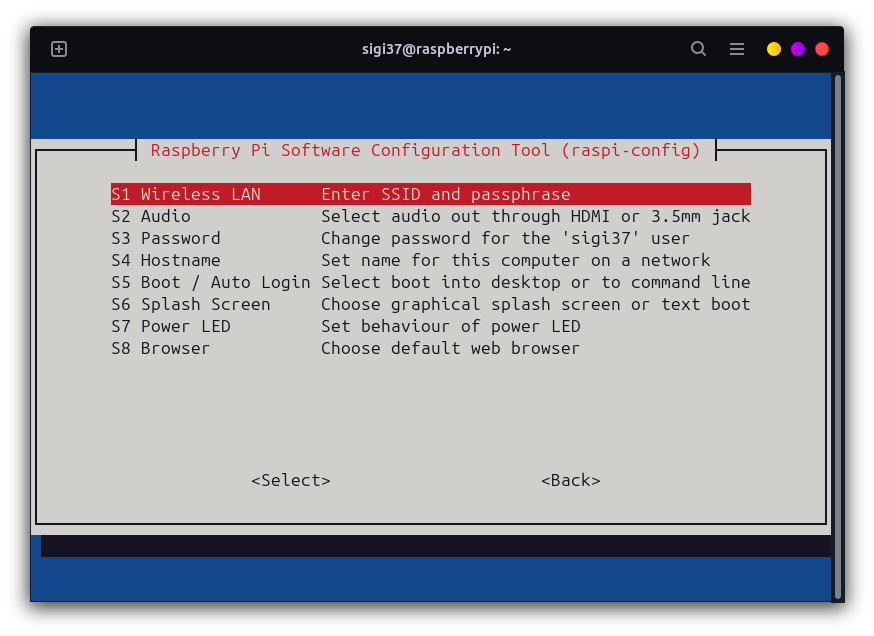
\includegraphics[scale=0.37]{img/raspi_config_wifi.png}

Then, you can enable the SSH connection in the Interface panel from the main menu.

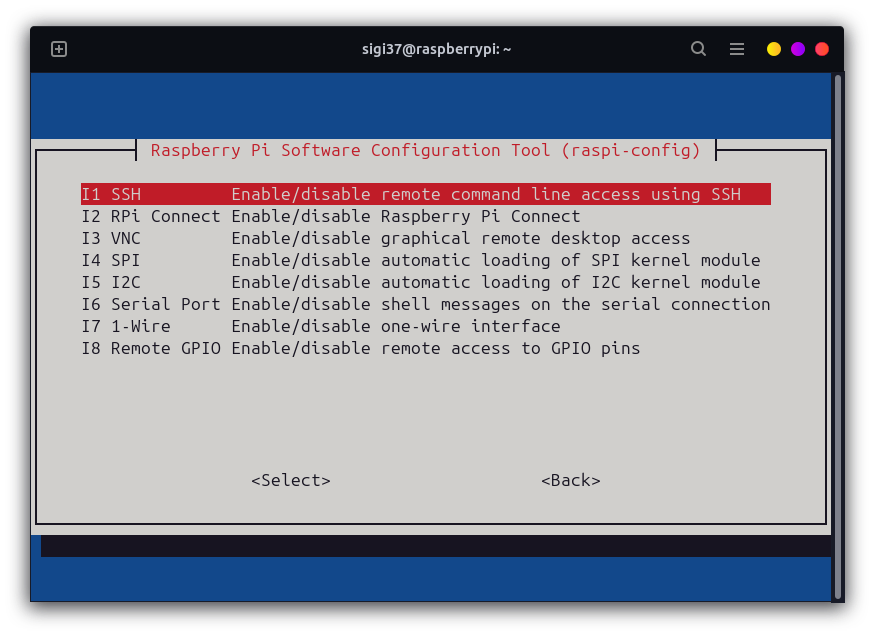
\includegraphics[scale=0.37]{img/raspi_config_ssh.png}

After exiting, you can check the IP address of the Raspberry Pi using the command:
\texttt{ip a show}

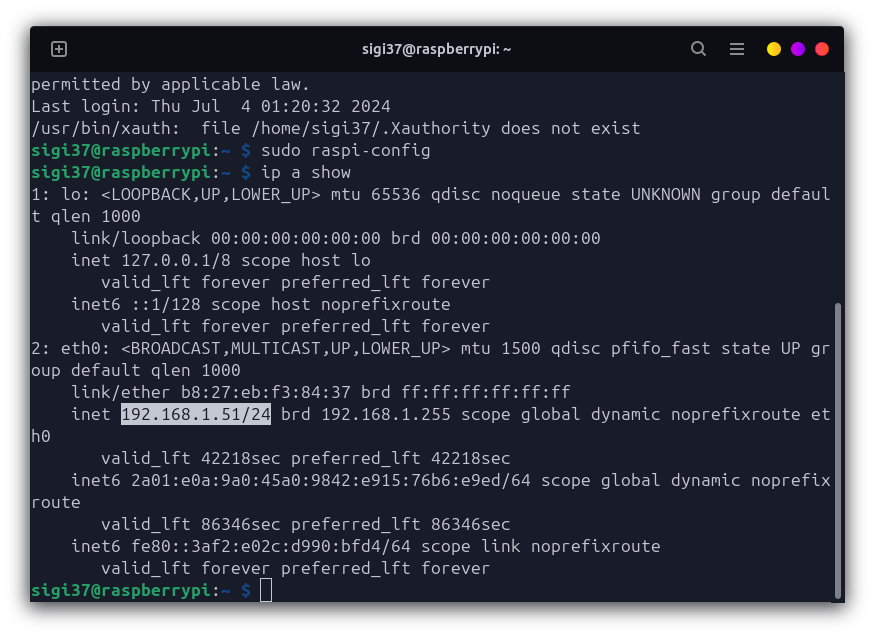
\includegraphics[scale=0.37]{img/ip_a_show.png}

The IP 127.0.0.1 is the loopback, it is not what we are looking for.
If you are connected on a normal network, you should see an IP
starting with 192.168 or 10.0, but if your network is complex, then your IP address might
be entirely different.

In my case, the IP is highlighted. In my case, it is below eth0 because I am connected via
Ethernet.

Then, you should be able to connect from your computer using the command:
\texttt{ssh <username>@<IP address>}

You should be prompted for the password if you haven't generated an ssh key.

\subsubsection{Check}

You should be connected to the Raspberry Pi, and you should be able to run commands on it.
For the following steps, you will need to type commands on the Raspberry Pi, so if you are
connected through SSH, you can copy-paste the commands from your computer to the Raspberry Pi.
Note: the copy-paste method on a terminal can be either \texttt{Ctrl+Shift+C} or
\texttt{Ctrl+C}, depending on the terminal and the OS(idem for paste with V).

If you have a keyboard and a screen, you can also type them directly.

Check that the Raspberry Pi is connected to the internet using the command:

\texttt{ping google.com}

then press \texttt{Ctrl+C} to stop the ping after a few seconds.

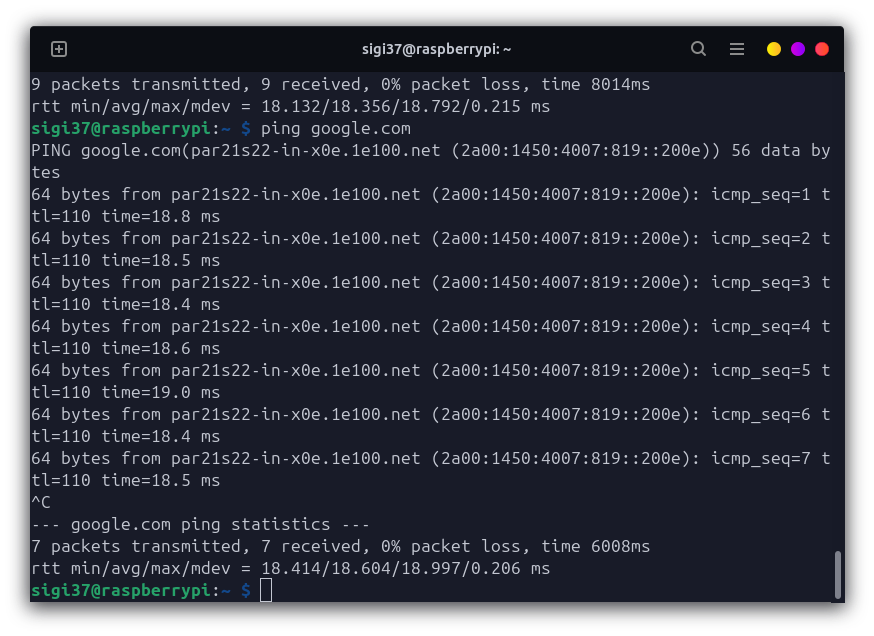
\includegraphics[scale=0.37]{img/ping_google.png}

The output should show that the packets are sent and received.

\subsubsection{Increasing the size of the root partition and updating the system}

The root partition of the Raspberry Pi is small by default, so we will increase it.

In the \texttt{sudo raspi-config} menu, you can find the option to expand the filesystem in the
Advanced Options panel. This will expand the root partition to the maximum size of the SD card.
Rebooting the Raspberry Pi is required to apply the changes. It should be done automatically after
you exit raspi-config.

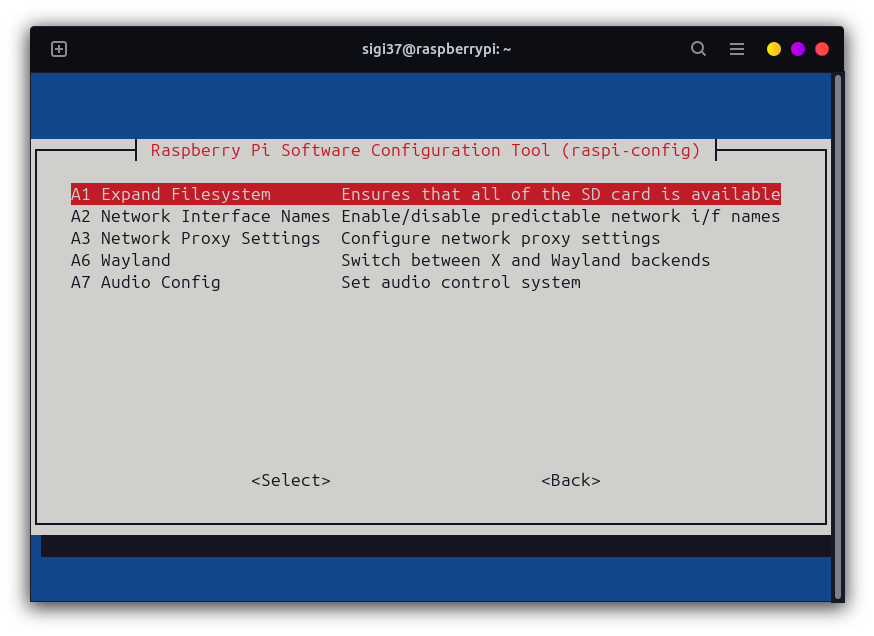
\includegraphics[scale=0.37]{img/raspi_config_expand.png}

Then we will refresh the repositories using the command:

\texttt{sudo apt update}

If the network is unreachable, the command will fail.

Then update the packages using the command:

\texttt{sudo apt upgrade}

It should take some time, the download is quite big.

\subsubsection{Check}

We will check that the raspberry pi has available space using the command:

\texttt{df -h}

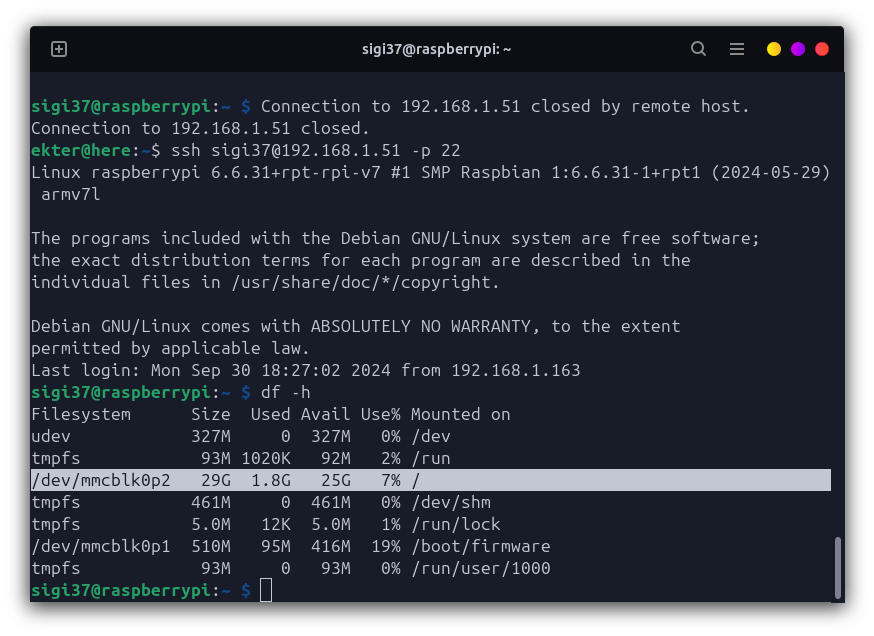
\includegraphics[scale=0.37]{img/df_h.png}

The line with \texttt{/} should show a size close to the size of the SD card, and a low usage.

\subsubsection{Setting up Python, git, and the I2C interface}

Python should already be installed, but just in case:

\texttt{sudo apt install python3-full python3-venv python3-pip}

If you install pip like this, you can use it with the command \texttt{pip}.
Sometimes it is referred to as \texttt{pip3}, but it is the same command.

Install git:

\texttt{sudo apt install git}

And OpenBlas needed to run numpy, clarabel, and most numerical libraries:

\texttt{sudo apt install libopenblas-dev}

We will also need the I2C interface to communicate with the Balboa board, so let's activate it
on rapsi-config.

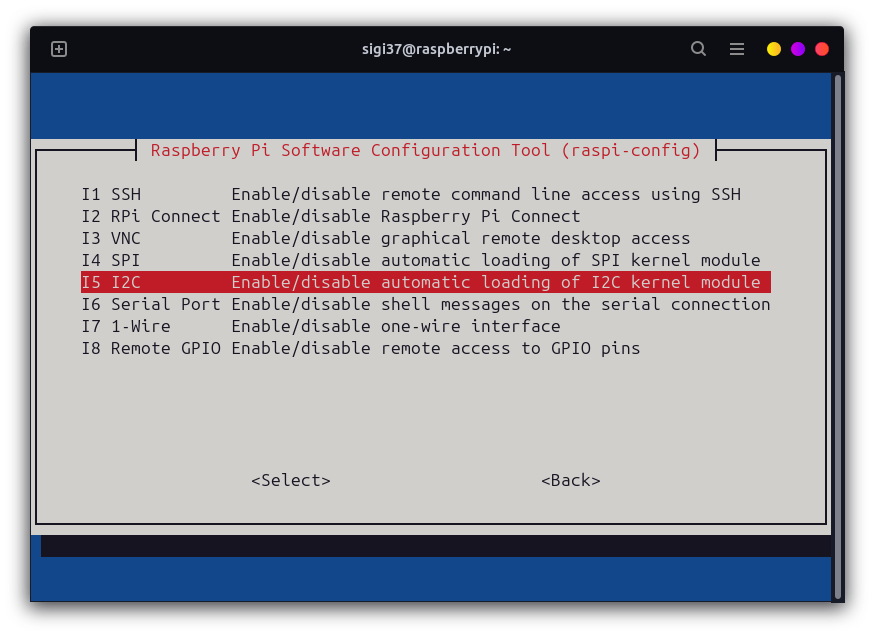
\includegraphics[scale=0.37]{img/rapsi_config_i2c.png}

We will also need to enable the remote GPIO server.

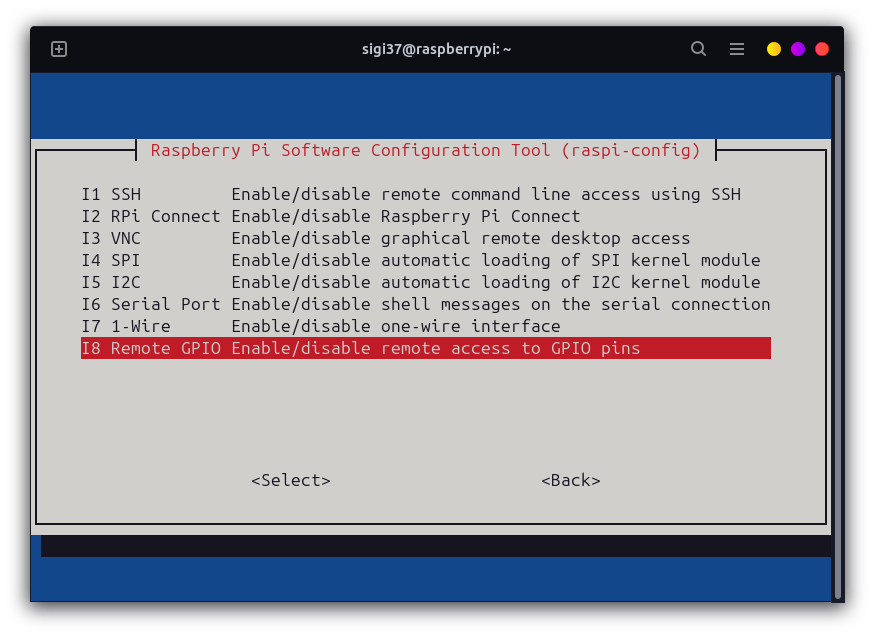
\includegraphics[scale=0.37]{img/raspi_config_rgpio.png}

We will then reboot to complete the changes.

\texttt{sudo reboot}

\subsubsection{Check}

Check the version of Python using the command:

\texttt{python3 --version}

The version of pip:

\texttt{pip3 --version}

And the version of git:

\texttt{git --version}

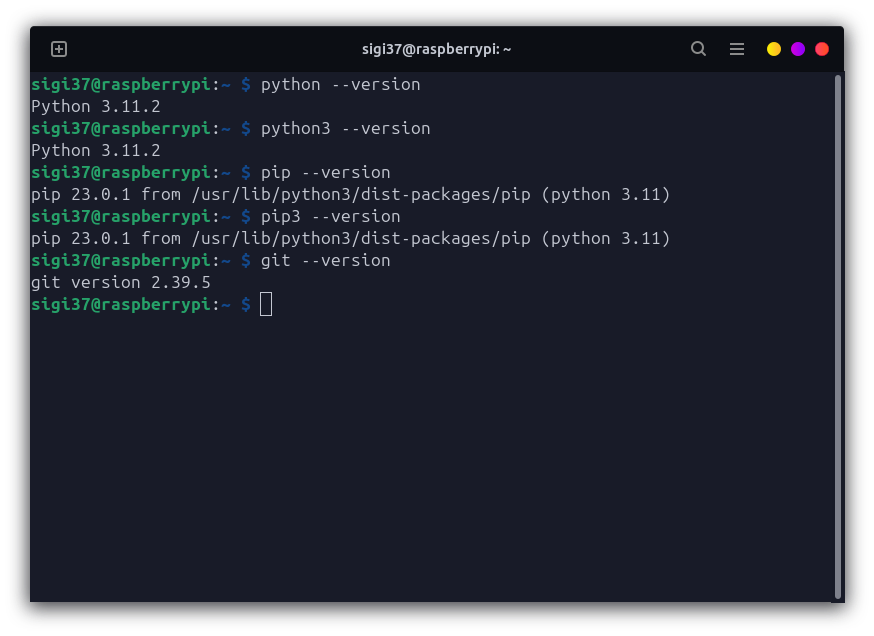
\includegraphics[scale=0.37]{img/all_versions.png}

\subsubsection{Cloning the sigi repository}

We will now clone this repository to get the code of the Sigi.

If you want to use different code, you can clone it instead, or just create a new repository.

I recommend you to make a fork of this repository and clone it, so you can push your changes
directly without having to make a pull request every time, but for now, we will just clone it.

\texttt{git clone} will create a folder with the name of the repository in the current directory.
Change the directory if needed using the \texttt{cd} command.

\texttt{git clone https://github.com/Ekter/sigi.git}

Or you can use the ssh version if you have generated an ssh key and added it to your Github
account:

\texttt{git clone git@github.com:Ekter/sigi.git}
(replace by your repository if you have created one)

If you need advise on how to use git, here is a nice tutorial:
\href{https://www.freecodecamp.org/news/learn-the-basics-of-git-in-under-10-minutes-da548267cc91/
}{Git tutorial by freecodecamp}

\subsubsection{Check}

Let's move inside the freshly cloned repository:

\texttt{cd sigi}

We should be able to see the files of the repository using the command:

\texttt{ls}

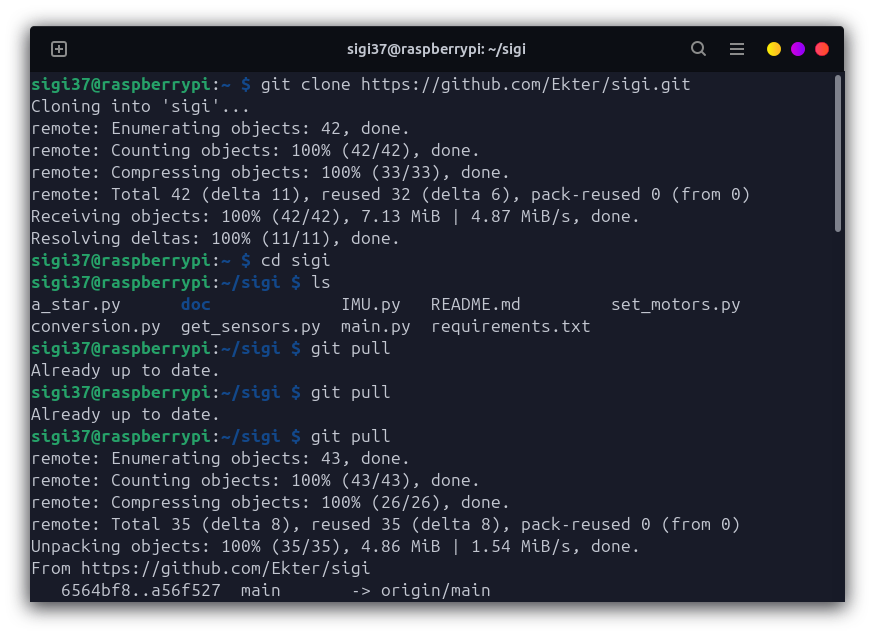
\includegraphics[scale=0.37]{img/git_worked.png}

\subsubsection{Creating the virtual environment and installing the dependencies}

We will now create a virtual environment to install the dependencies of the project.

Still in the repository, we will use the command:

\texttt{python3 -m venv .venv}

This will create a folder named \texttt{.venv} in the repository, containing the virtual
environment.

Then we will activate the virtual environment using the command:

\texttt{source .venv/bin/activate}

The prompt should change to show that the virtual environment is activated.

To deactivate the virtual environment, you can simply run \texttt{deactivate}, but don't do it
for now.

Then we will install the dependencies using the command:

\texttt{pip install -r requirements.txt}

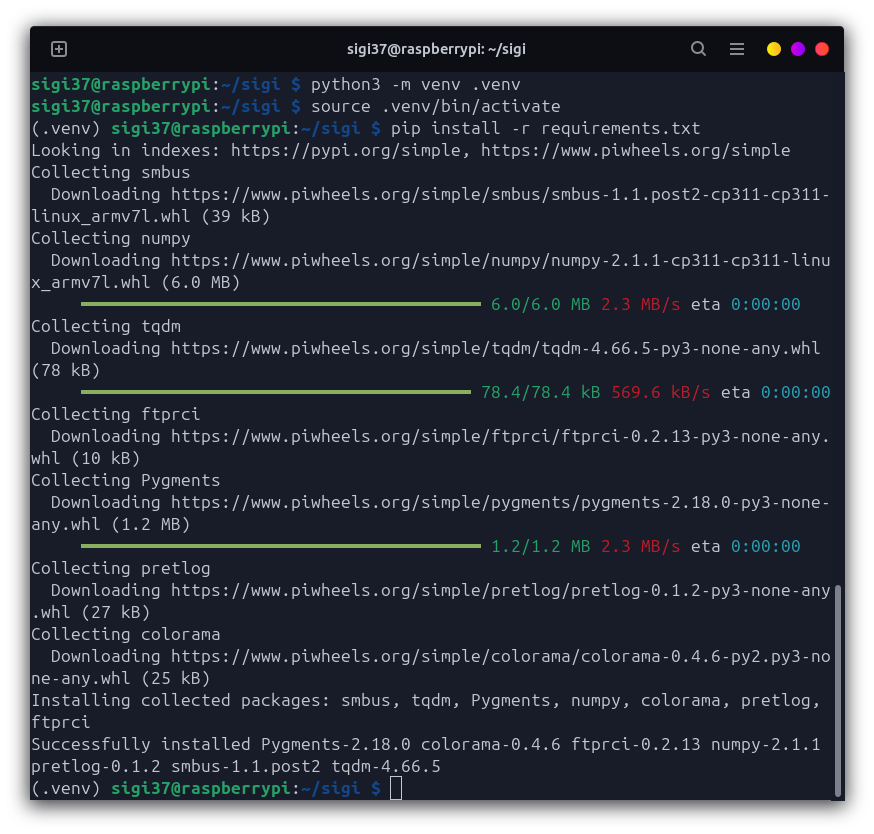
\includegraphics[scale=0.37]{img/venv_activated.png}

Now we should be able to run the code of the Sigi.

If you prefer to use Jupyter notebooks, you should install IPython:

\texttt{pip install ipython}

\subsubsection{Check}

We will run the code to check if everything is working.

To just read the sensors data, we will use the script:

\texttt{python3 get\_sensors.py}

It should print the values of the sensors.

Quit the script using \texttt{Ctrl+C}.

To make the robot balance itself, we will use the main script described in the software section:

\texttt{python3 main.py}

Maybe one day this will work.

\subsection{Working on the code}

There are several ways to edit the code of the Sigi. The easiest way is to edit the files from the
terminal using nano for example:

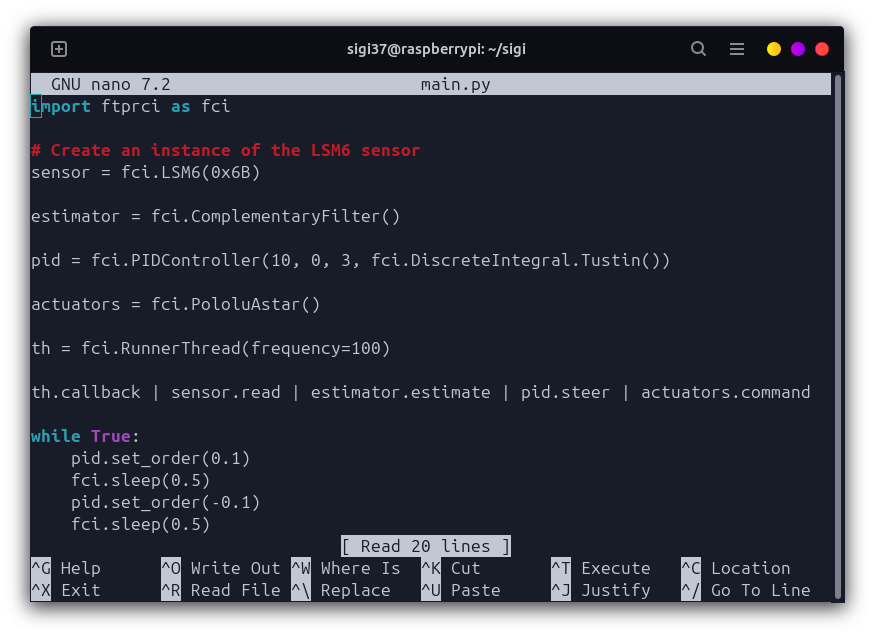
\includegraphics[scale=0.37]{img/nano_main.png}

But this is really inconvenient.

Another way is to code from your computer(following the same instructions to clone the repo), push
changes to github, and pull them from the Raspberry Pi.

It feels to be the natural way to do it in my opinion. However, being able to quickly edit the
code from the Raspberry Pi can be useful, so I advise you to get an editor on the Raspberry Pi.

The most convenient in this domain is Visual Studio Code: you can have it running on your computer,
and connected to the raspberry pi to edit the code directly on the Raspberry Pi.

The only downside is that you will have two windows of VS Code running all the time (one on your
computer, and one on the Raspberry Pi), but it is not a big deal.

Furthermore, VS Code has plenty of capabilities, like the git integration, allowing you to manage
your commits directly from the editor.

The cherry on the cake is that all we need to use VS Code remotely is the SSh connection!

\subsubsection{Installing Visual Studio Code, some extensions, and connecting remotely}

If you haven't installed it yet, \href{https://code.visualstudio.com/}{download Visual Studio Code}
on your computer.


In the extensions tab, you can install the Remote - SSH extension.
I also advise you to install some extensions:

\begin{itemize}
    \item Python for easy Python coding and debugging;
    \item Jupyter for Jupyter notebooks;
    \item Gitlens for git integration;
    \item Trunk for linting and formatting management;
    \item Black Formatter and isort for python code formatting;
    \item vscode-pdf for pdf reading;
    \item or LaTeX Workshop for LaTeX writing;
    \item Markdown All in One for markdown editing;
    \item rainbow-CSV or Excel Viewer for better readability of CSV files;
    \item indent-rainbow for better readability of code;
    \item Remote Explorer if you plan to connect to multiple devices;
    \item Doki Theme for nice visual themes;
\end{itemize}

If several extensions show up, choose the one from Microsoft, or the one with the biggest number of
downloads.

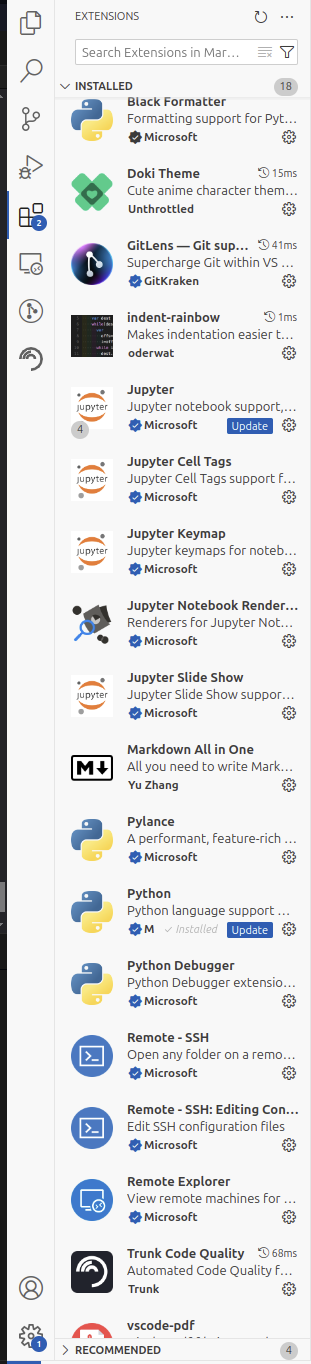
\includegraphics[scale=0.2]{img/vsc_exts.png}

Now let's connect to the Raspberry Pi using the Remote - SSH extension.

Click on the icon with the \texttt{><} sign(remote button) and choose Remote-SSH: Connect to Host.
Add a new ssh host, and enter the exact command you used to connect to the Raspberry Pi.

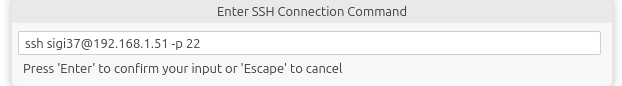
\includegraphics[scale=0.5]{img/vsc_ssh.png}

Update the default configuration file unless you have specific needs for it.

Then you can click on the remote button again, and click connect to host. The host you have just
added will be labelled by its IP address, but you can change it in the configuration file,
by choosing the option Configure SSH Hosts.

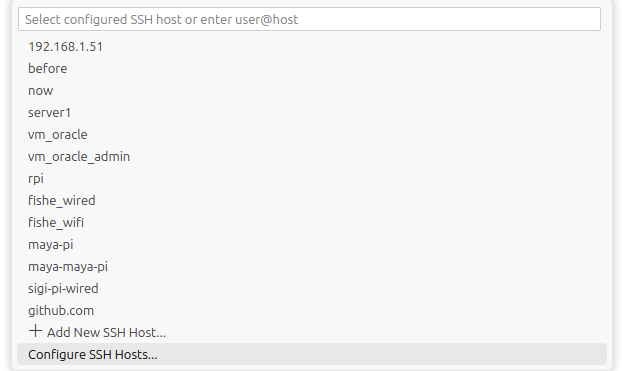
\includegraphics[scale=0.5]{img/vsc_ssh2.png}

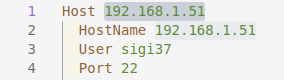
\includegraphics[scale=0.5]{img/vsc_ssh_edit.png}

Warning: the option to change is Host, not HostName. HostName is the address of the host(IP,
domain...). You should not need the Port field if you have not changed your system's default ssh
port.

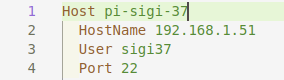
\includegraphics[scale=0.5]{img/vsc_ssh_edit2.png}

Now let's actually connect to the Raspberry Pi by clicking on the host in the connect list.

A new window should open, and after VS Code has installed the server on the Raspberry Pi, you
should be connected, and the name on the remote button should be \texttt{SSH: <your host>}.

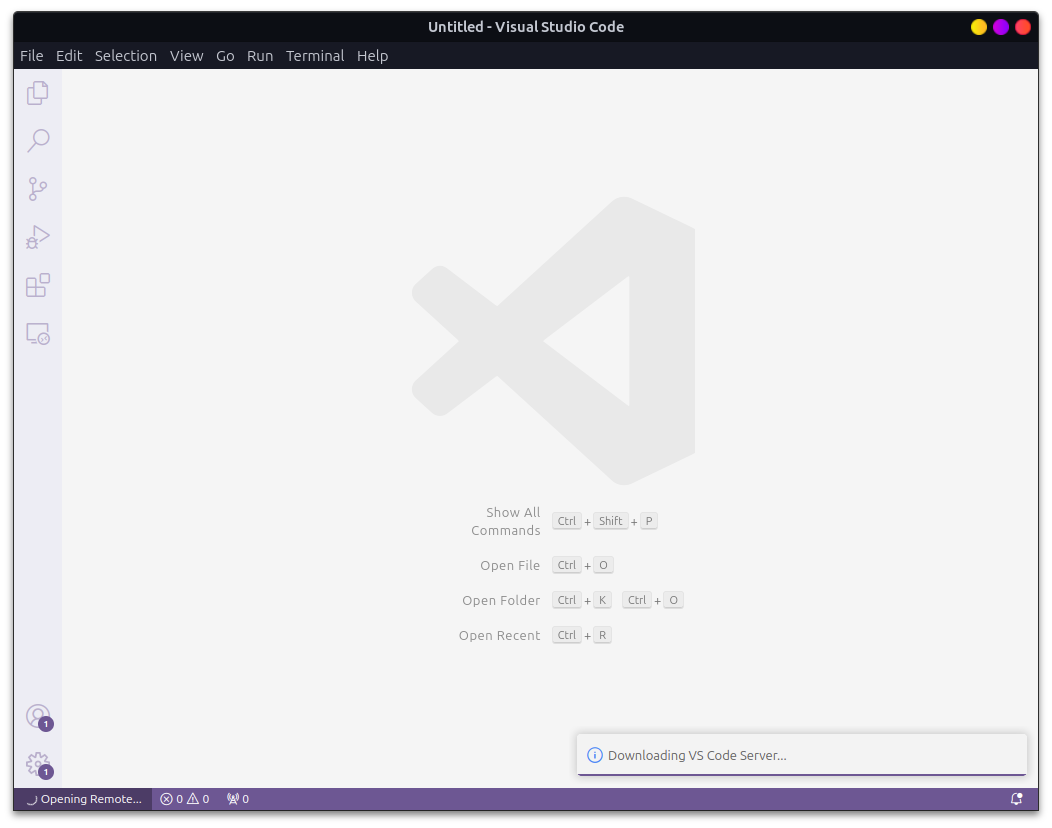
\includegraphics[scale=0.3]{img/vsc_ssh_connecting.png}

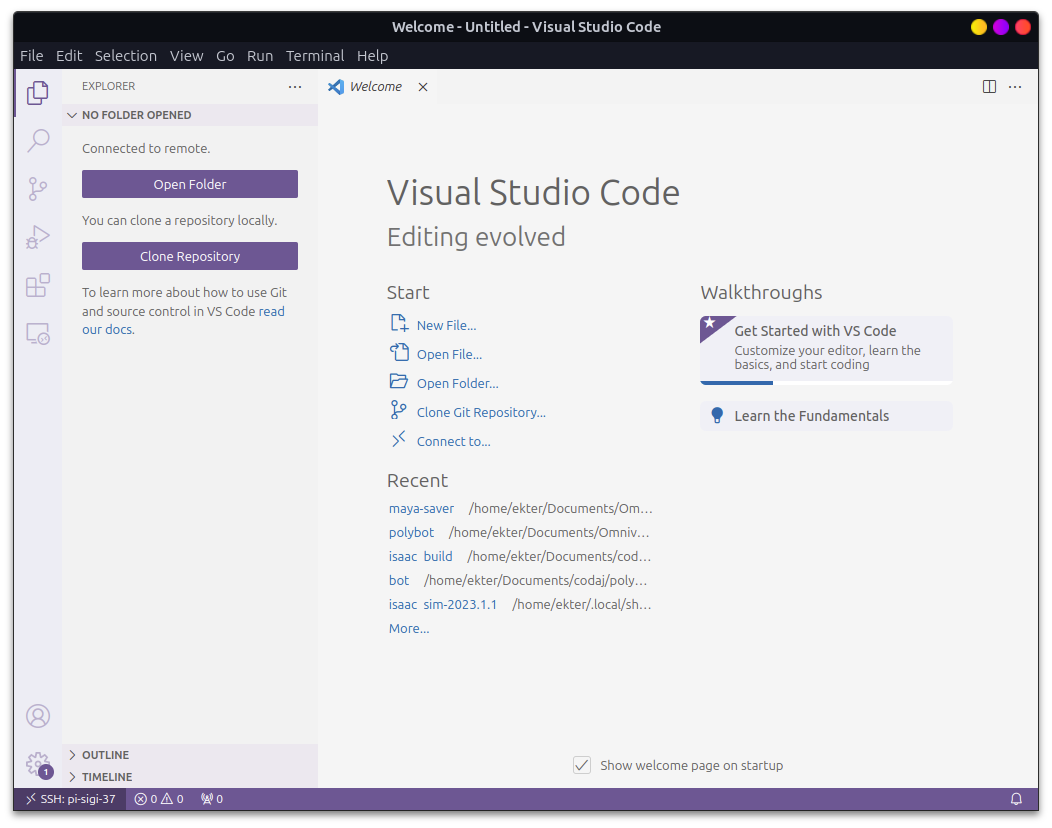
\includegraphics[scale=0.3]{img/vsc_ssh_connected.png}

If it doesn't work, check that the ssh command works in the terminal. Also, you will need the
Raspberry Pi to be connected to the internet, at least for the first connection and when VS Code
updates.

Now we can work as usual on the Raspberry Pi, but with the comfort of VS Code.

You can open a terminal on the Raspberry Pi directly from VS Code, and run the commands we have
used for checks directly from there.

If they did not re-install automatically on the remote window, you can install the extensions
again, especially the Python extension.

Click Open Folder to open the folder we cloned earlier.

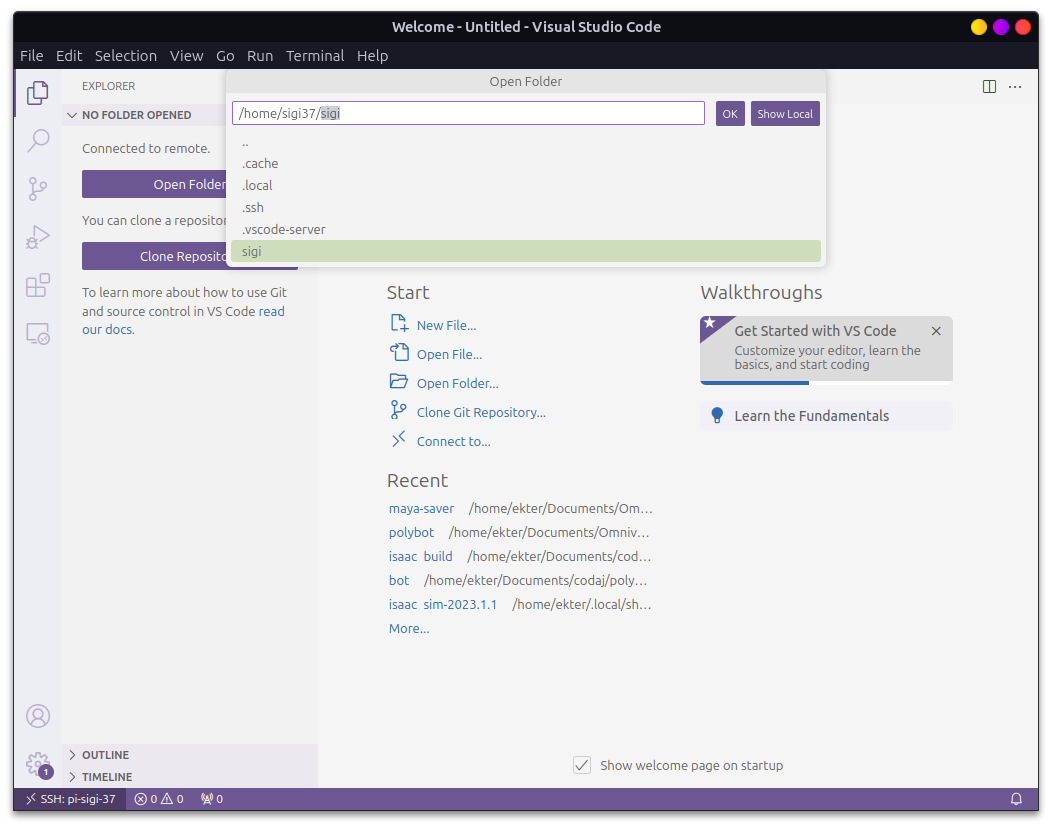
\includegraphics[scale=0.3]{img/vsc_open_folder.png}

You can open the file \texttt{main.py} or \texttt{get\_sensors.py} and debug them directly using
f5 or the options of the green play button.

Check that the Python interpreter is the virtual environment we have created on the bottom bar:
it should say something like \texttt{'.venv': venv}.

You can create a launch.json file to configure the debugging options, and make launching easier.
All the configuration is done automatically by VS Code, but you can change it if you want.

Here is how it should look like when you are debugging if you have an error:

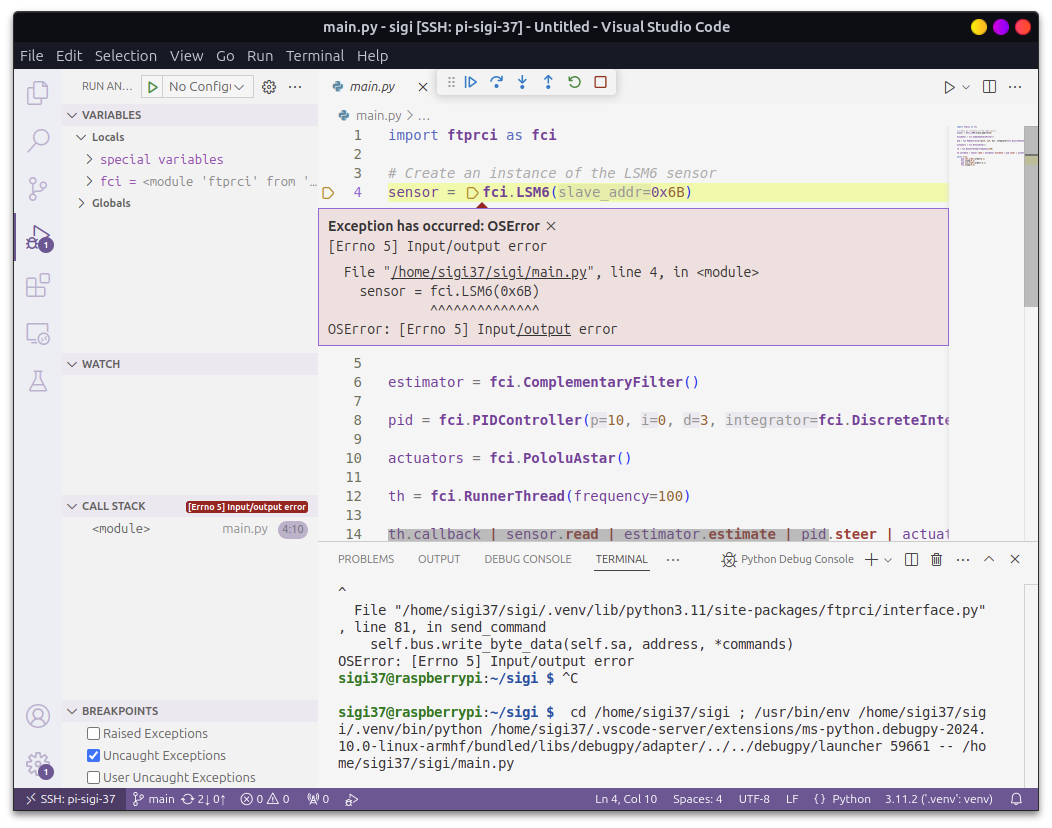
\includegraphics[scale=0.3]{img/vsc_debug.png}

Using git, you can keep your code up to date between your computer and the Raspberry Pi.
If you edit the code, you can push the changes to the repository using the git panel, or using the
terminal.

You should be all set to work on the Sigi now!

If you have any questions or suggestions on how to improve this tutorial, do not hesitate to open
an issue or a PR on the Github repository.

\end{document}

% todo put figures
% todo choose between we and you for tuto
